\documentclass{article}
\usepackage{geometry}
\usepackage{float}
\usepackage[T1]{fontenc}
\usepackage[polish]{babel}
\usepackage[utf8]{inputenc}
\usepackage{graphicx}
\graphicspath{ {./images/} }

\geometry{
 a4paper,
 total={170mm,257mm},
 left=20mm,
 top=20mm,
}

\title{Analiza i przetwarzanie dźwięku - Projekt 2}
\date{04/05/2020}
\author{Mateusz Śliwakowski}

\begin{document}
  \pagenumbering{gobble}
  \maketitle
  \pagenumbering{arabic}
  
\section{Treść zadania}
Celem zadania było zaimplementowanie programu, który wczytuje plik audio a następnie przeprowadza jego analizę widmową. Należało umożliwić użytkownikowi wykonanie transformaty Fouriera całego sygnału oraz ramek o długości $2^N$ zaczynających się w dowolnym miejscu w sygnale. Dla ramek należało umożliwić zastosowanie funkcji okienkowych:
\begin{itemize}
\item okna prostokątnego,
\item okna Hamminga,
\item okna van Hanna.
\end{itemize}
Kolejną funkcjonalnością, którą była wymagana było rysowanie spektogramu dla sygnału. Należało pozwolić na zmianę długości ramek, wybór okna oraz zmianę procentu nakładania się ramek. Ostatnim wymaganiem było zaimplementowanie wykresu częstotliwości krtaniowej za pomocą cepstrum.

\section{Opis aplikacji}

Aplikację zdecydowałem się wykonać w języku \textit{C\#} w środowisku \textit{WinForms}. Całość zacząłem od zaprojektowania wyglądu interfejsu użytkownika.

\begin{figure}[H]
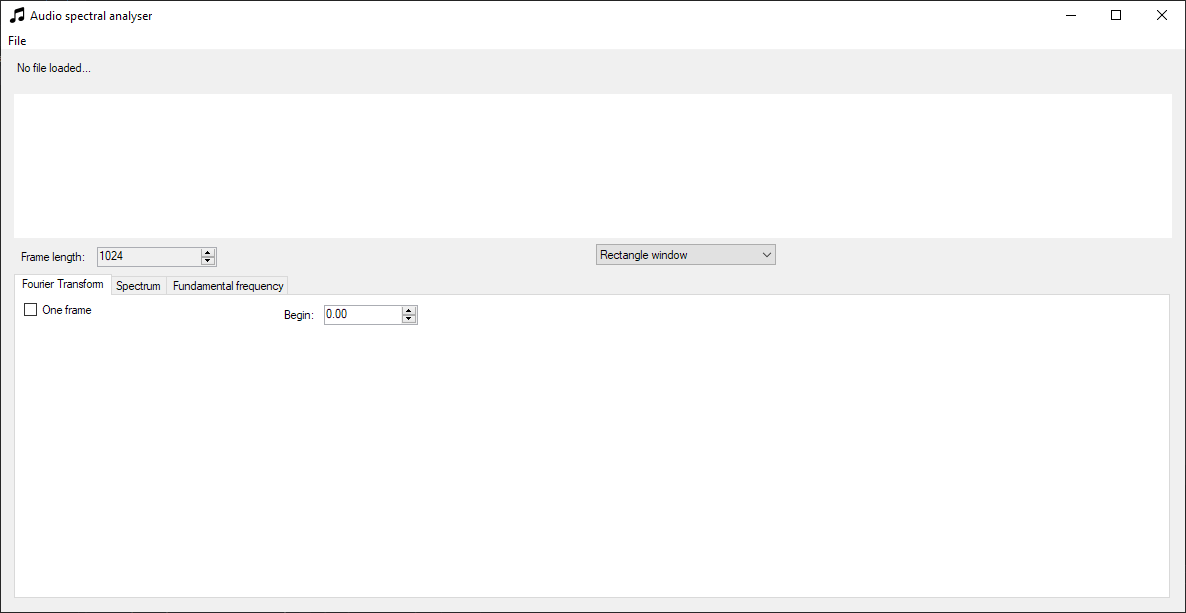
\includegraphics[width=\textwidth]{scr1.png}
\caption{Interfejs użytkownika}
\label{fig:interface}
\end{figure}

Do wczytywania plików audio użyłem biblioteki \textit{NAudio}. Bez problemu umożliwia ona ładowanie przebiegu audio oraz informacji o ścieżce takich jak długość, czy sample rate. Do rysowania wykresów użyłem, w przeciwieństwie do poprzedniego projektu, biblioteki \textit{OxyPlot}, która okazała się dużo bardziej komfortowa w użyciu oraz małym nakładem pracy zapełniła podstawowe funkcjonalnosci takie jak przybliżanie i oddalanie wykresu, przesuwanie, dodawanie etykiet osi. Na początku do obliczania FFT używałem funkcji zaimplementowanych w bibliotece \textit{NUnit}, jednak ze względu na niezadowalające rezultaty zmieniłem ją na \textit{MathNet.Numerics}. Dostarczyła mi ona funkcjonalności wystarczające do obliczania FFT, odwrotnej FFT oraz stosowania funkcji okna.

\section{Zaimplementowane metody}
\subsection{Transformata Fouriera}
\label{subsection:FFT}

Transformata Fouriera pozwala na przejście z dziedziny czasu na dziedzinę częstotliwości dla sygnału audio. Jako, że cyfrowy sygnał audio opisany jest funkcją dyskretną, należy użyć Dyskretnej Transformaty Fouriera. Jej naiwna implementacja ma złożoność $O(N^2)$, zatem w praktycznych zastosowaniach korzysta się z \textit{Fast Fourier Transform}, czyli szybkiej transformacji Fouriera, której złożoność jest równa $O(Nlog_2N)$ co pozwala nawet na analizę sygnałów w czasie rzeczywistym. FFT jako argument przyjmuje ramkę o długości $2^N$ i zwraca wartości w przekształconej dziedzinie. W implementacji należało zadbać, aby funkcja obliczająca FFT zawsze otrzymała tablicę o odpowiedniej długości, prawidłowy podział sygnału na ramki oraz skalowanie osi na wykresie. Warto zwrócić uwagę, na fakt iż na wykresie należy wyświetlić połowę wynikowej tablicy, co odpowiada częstotliwościom od zera do połowy częstotliwości próbkowania. Fakt ten wynika z własności częstotliwości Nyquista.
\\

Próbki FFT mogą zostać przekształconę funkcją okna. Funkcje te przyjmują wartości od 0 do 1, są symetryczne względem osi OY, przeważnie maleją począwszy od punktu 0 w obie strony. Przed poddaniem sygnału transformacji wartości są mnożone przez odpowiednie wartości funkcji okna. Pozwala to na uniknięcie zjawiska wycieku widma i poprawienie wyniku działania FFT. 

\subsection{Spektogram}

W szerszym zakresie analizę sygnału audio w dziedzinie częstotliwości umożliwia spektogram. Przedstawia on spektrum sygnału, zmieniające się w czasie. Aby narysować spektogram poddajemy analizie kolejne ramki o podanej długości, biorąc pod uwagę ich wzajemne nakładanie. Następnie wartości po przekształceniu wpisujemy do wykresu w osi pionowej. Do funkcji FFT brane są wszystkie parametry, wymienione w \ref{subsection:FFT}.

\subsection{Częstotliwość tonu podstawowego mowy}

Ostatnim i zdecydowanie najtrudniejszym zagadnieniem, było wykrywanie częstotliwości tonu podstawowego mowy za pomocą cepstrum. Dla pojedynczej ramki, ton podstawowy obliczałem w następujący sposób:
\begin{enumerate}
\item Oblicz FFT dla ramki.
\item Przekształć wynikową tablicę za pomocą następującej funkcji $log|t|$.
\item Przeprowadź odwrotną FFT na tablicy z 2.
\item W przedziale odpowiadającym częstotliwościom od 50Hz do 400Hz znajdź indeks $x$, dla którego wartość w tablicy jest maksymalna.
\item Przekształć indeks $x$ na odpowiadający mu czas $t$.
\item $F_0 = \frac{1}{t}$
\end{enumerate}

Algorytm ten powtarzałem dla kolejnych ramek, wyznaczanych analogicznie jak dla spektogramu. Wynik przedstawiłem na wykresie liniowym.

\section{Wyniki działania programu}

Sprawdźmy, czy dla sygnału o stałej częstotliwości fali uzyskamy poprawny wynik. W tym celu skorzystałem z narzędzia generującego fale sinusoidalne o zadanej częstotliwości. Dla 400Hz uzyskałem następujący rezultat:

\begin{figure}[H]
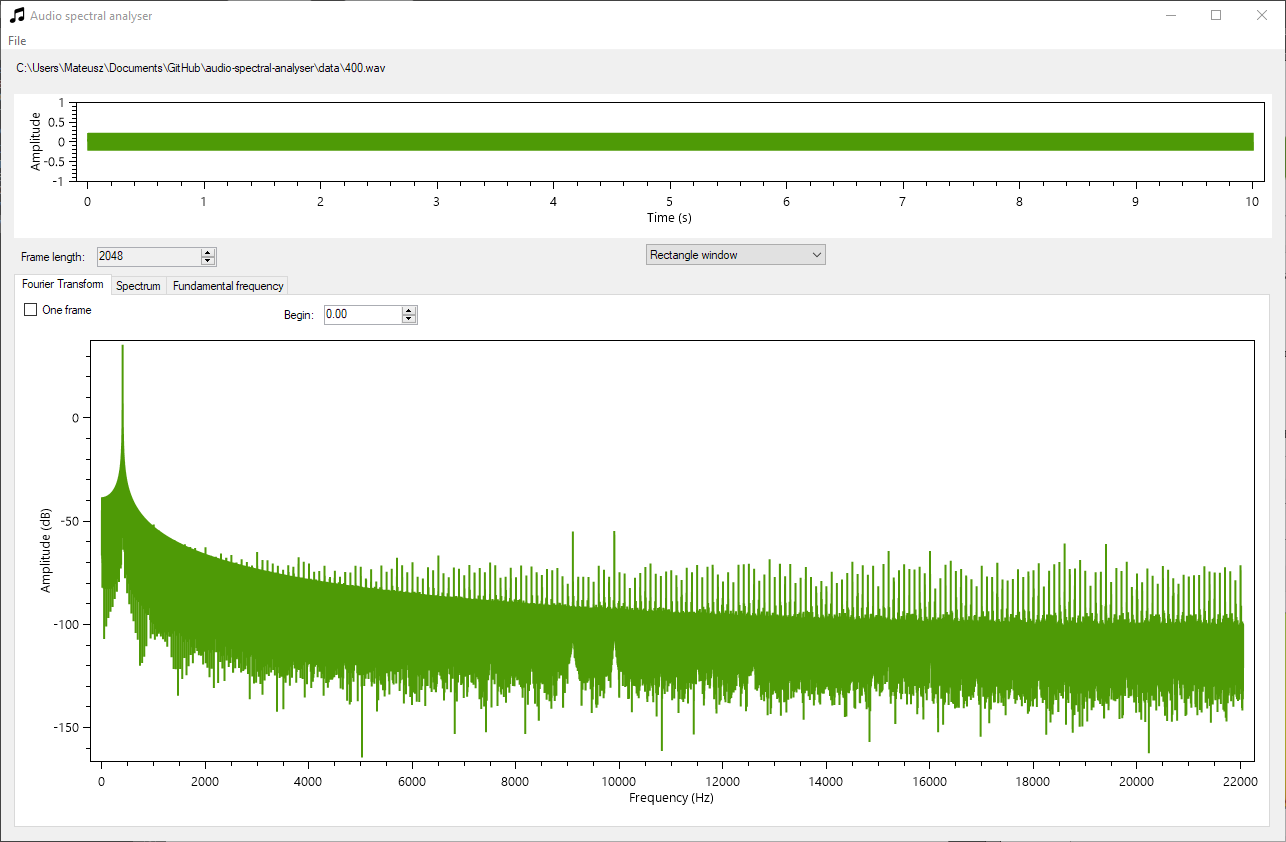
\includegraphics[width=\textwidth]{scr2.png}
\caption{Analiza dla sztucznie wygenerowanej próbki 440Hz}
\label{fig:interface}
\end{figure}

Najwyższa wartość przypada w spodziewanym miejscu, lecz całość wykresu jest mocno zaszumiona. Zobaczmy teraz jak funkcja okna wpłynie na kształt wykresu:

\begin{figure}[H]
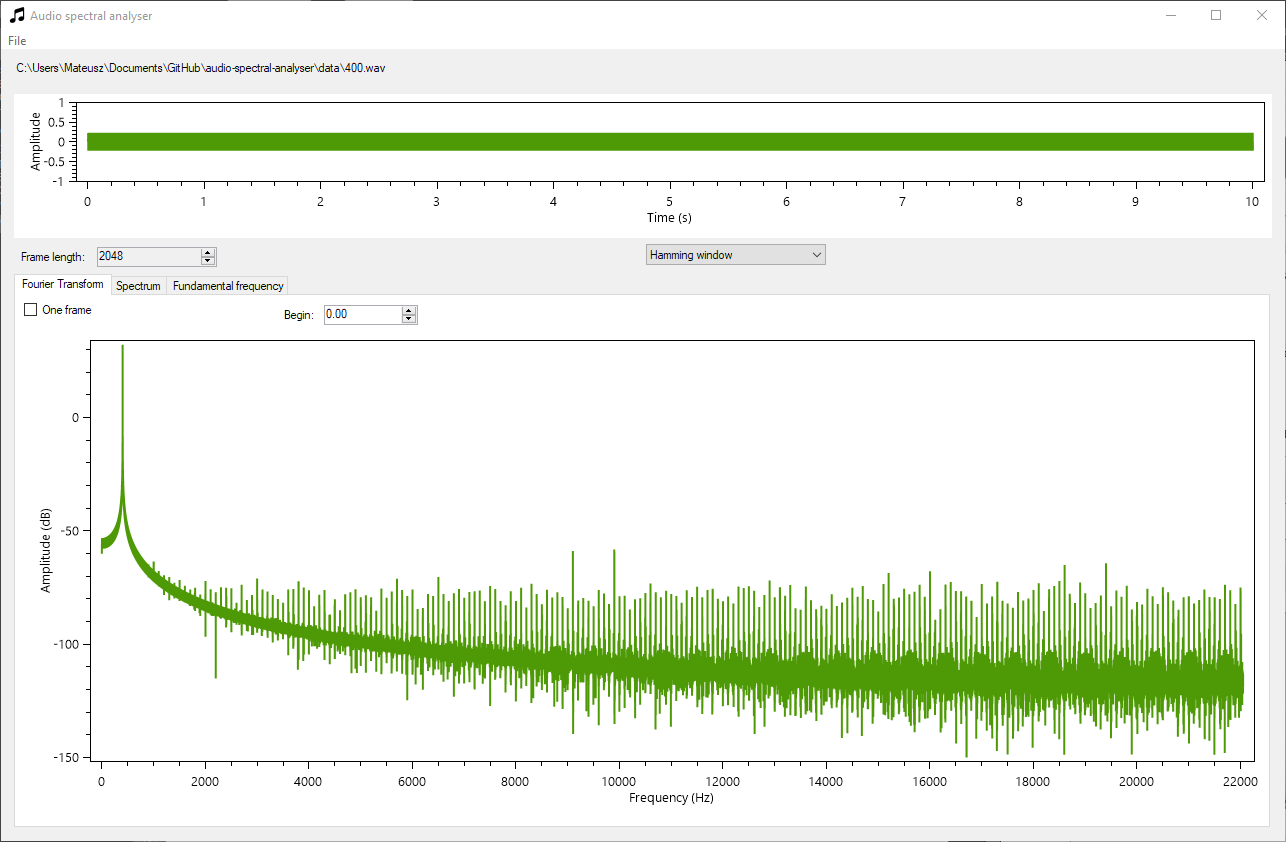
\includegraphics[width=\textwidth]{scr3.png}
\caption{Analiza dla sztucznie wygenerowanej próbki 400Hz, okno Hamminga}
\label{fig:interface}
\end{figure}

Jak widać wynik jest widocznie odszumiony, zwłaszcza w okolicach jego maksymalnej wartości. Podobne wyniki otrzymamy, dzięki zastosowaniu okna van Hanna:

\begin{figure}[H]
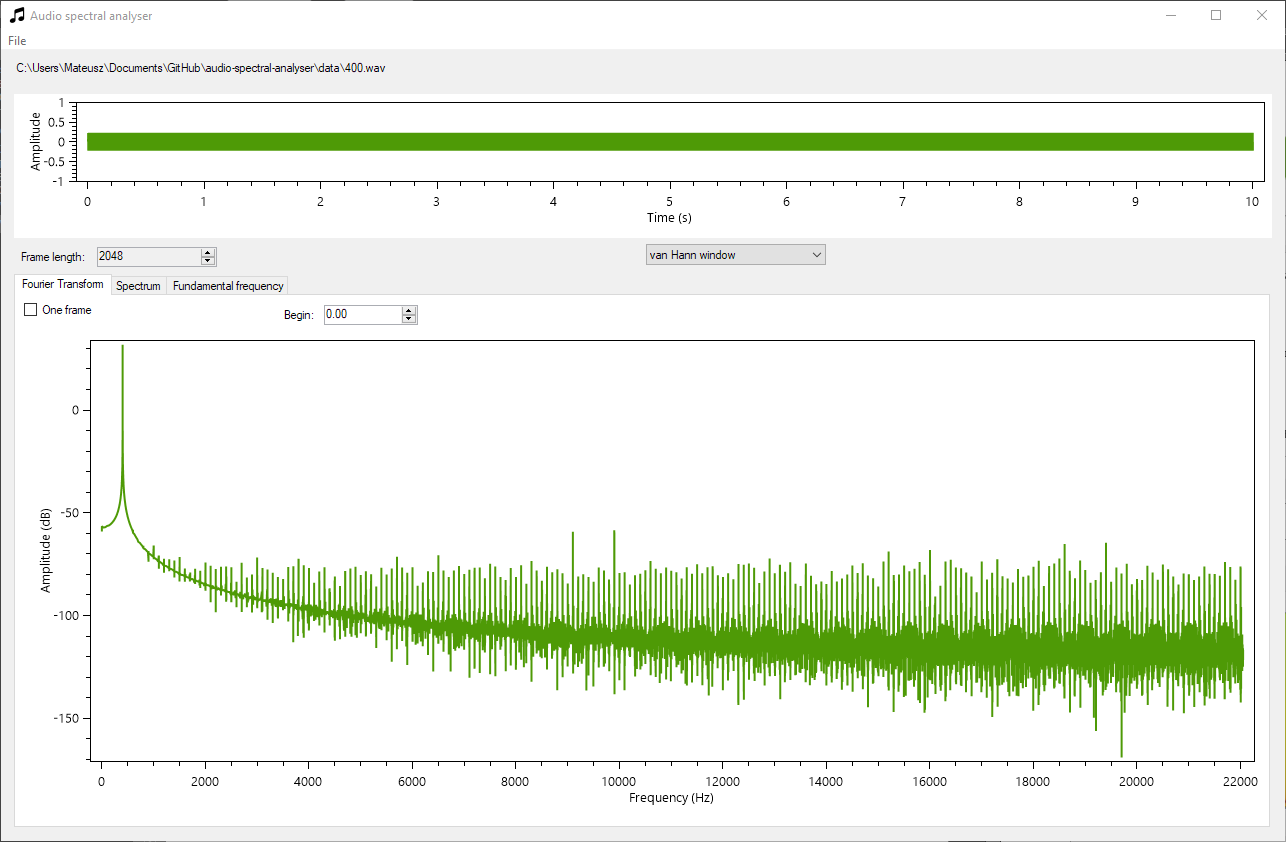
\includegraphics[width=\textwidth]{scr4.png}
\caption{Analiza dla sztucznie wygenerowanej próbki 400Hz, okno van Hanna}
\label{fig:interface}
\end{figure}

Zobaczmy jak wygląda spektogram dla takiego pliku. Ponownie, znacznie lepszy rezultat uzyskujemy stosując funkcję okna:

\begin{figure}[H]
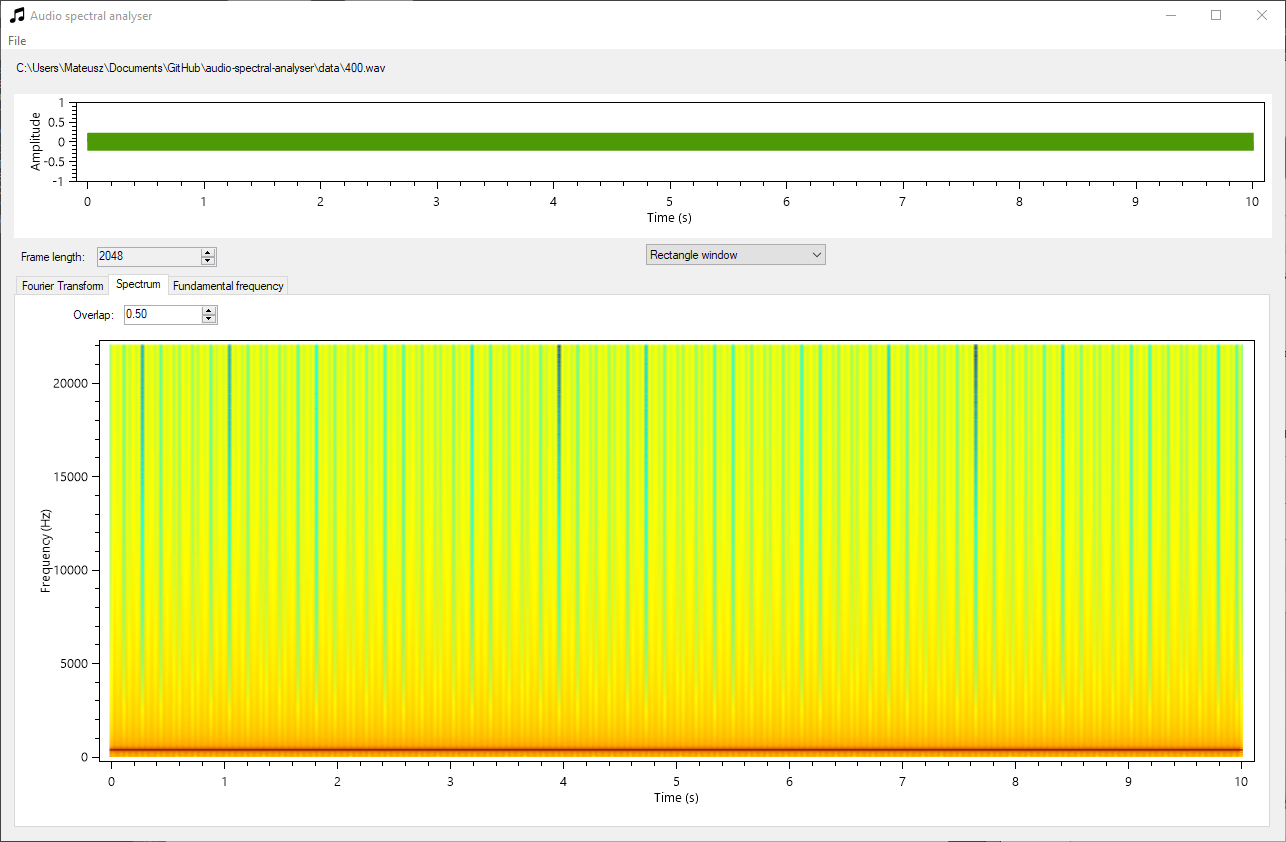
\includegraphics[width=\textwidth]{scr5.png}
\caption{Analiza dla sztucznie wygenerowanej próbki 400Hz, spektogram}
\label{fig:interface}
\end{figure}

\begin{figure}[H]
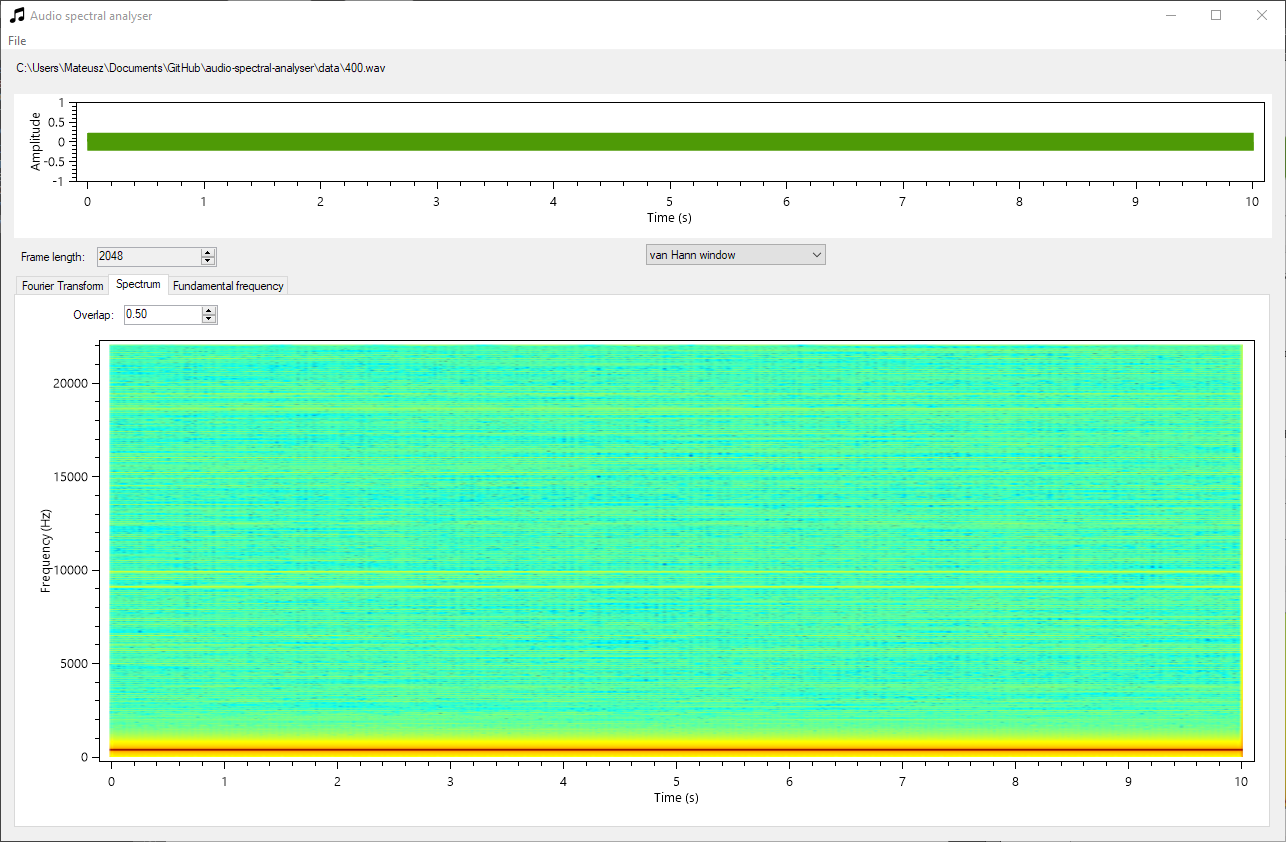
\includegraphics[width=\textwidth]{scr6.png}
\caption{Analiza dla sztucznie wygenerowanej próbki 400Hz, spektogram, okno van Hanna}
\label{fig:interface}
\end{figure}

\section{Wnioski}

\begin{figure}[b]
\centering
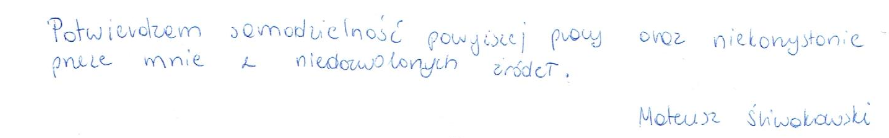
\includegraphics[width=5in]{bottom.png}
\end{figure}

\end{document}

